%!TeX root = Chapter_Method
\documentclass[../../CompleteThesis/Complete_1stDraft.tex]{subfiles}
\begin{document}
This section contains a walk through of the method to back diffuse a given ice core depth series to attempt to restore as much of the original signal as possible. For now, the method has been developed for sections that has been dated to be between the two volcanic eruptions Laki and Tambora, as these are very well dated, and thus it is possible to find the optimal diffusion length to back diffuse with as the actual number of annual layers is exactly known for this data series. The method is easily modified for any other dated depth series, as what is needed is just the number of annual layers in the given data series.\\
Figure \ref{Fig:FlowchartDiffLen} shows a flowchart of the method used to estimate the diffusion length of a depth series with a preliminary guess of number of annual layers. In the following sections each of the steps in the method will be discussed more thoroughly and examples will be given, all based on the Greenlandic ice core drilled at Site A near Crete(REFERENCES!!!).
The method is built such that it takes two inputs - the isotopic depth series, and the specifications for the particular ice core - and uses these for the first preliminary computations needed to make a first, naïve guess of the diffusion length, $\sigma_0$.
This diffusion length is then used to deconvolute the data and give a first estimate of the number of peaks in the data series. If this number is different from the already specified number of annual layers - in this case 32 - then the diffusion length will be updated accordingly: If the counted number is higher(lower) than the actual number, the diffusion length is adjusted downwards(upwards) with $\Delta\sigma_2$ and the deconvolution and peak counting is performed again.
On the other hand, if the counted number is equal to the actual number, then the diffusion length is optimized to find the largest diffusion length which still gives the actual number of counted peaks. When this $\sigma_{\text{final}}$ is reached, the algorithm stops and returns the final diffusion length estimate along with the associated back diffused depth series.
\begin{figure}
	\begin{tikzpicture}[node distance=1.5cm, auto]
		\node(start) [startstop] {START};
		%----------------------------------------------------%
		\node(in1) [io, left of=start, xshift=-3.5cm] {Depth series};
		\node(in1pro1) [process, below of=in1, yshift=-0.5cm] {Spline interpolation};
		\node(in1pro2) [process, below of=in1pro1] {Spectral analysis};
		\node(in1pro3) [process, below of=in1pro2] {Wiener filter};
		%	\node(in1pro4) [process, below of=in1pro3] {\textbf{Frequency filters}};	
		
		\draw[arrow] (in1) -- (start);
		\draw[arrow] (start) |- (in1pro1);
		\draw[arrow] (in1pro1) -- (in1pro2);
		\draw[arrow] (in1pro2) -- (in1pro3);
		%	\draw[arrow] (in1pro3) -- (in1pro4);
		
		%----------------------------------------------------%
		\node(in2) [io, right of=start, xshift=3.5cm] {Core specs};
		\node(in2pro1) [process, below of=in2, yshift=-0.5cm] {Density profile};
		\node(in2pro2) [process, below of=in2pro1] {Diffusion profile};
		\node(in2pro3) [process, below of=in2pro2] {$\sigma_0$\textbf{ estimate}};
		
		\draw[arrow] (in2) -- (start);
		\draw[arrow] (start) |- (in2pro1);
		\draw[arrow] (in2pro1) -- (in2pro2);
		\draw[arrow] (in2pro2) -- (in2pro3);
		
		%----------------------------------------------------%
		\node(pro0) [process, below of=start, yshift=-4.5cm] {\textbf{Frequency Filters}};
		\node(pro1) [process, below of=pro0] {\large{\textbf{BACK DIFFUSE}}};
		\node(pro2) [process, below of=pro1] {Count N Peaks};
		\node(dec1) [decision, below of=pro2, yshift=-.5cm] {$N = 32$ ? };
		
		\draw[arrow] (in1pro3) -| (pro0);
		\draw[arrow] (in2pro3) -| (pro0);
		\draw[arrow] (pro0) -- (pro1);
		\draw[arrow] (pro1) -- (pro2);
		\draw[arrow] (pro2) -- (dec1);
		
		%----------------------------------------------------%	
		\node(pro3a) [process, below of=dec1, xshift=-3cm] {$\sigma = \sigma + \Delta \sigma_1 $};
		\node(pro3apro1) [process, below of=pro3a] {Back diffuse};
		\node(pro3apro2) [process, below of=pro3apro1]  {Count N peaks};
		\node(pro3apro3) [process, below of=pro3apro2, xshift=-2cm] {$\sigma_{\text{final}} = \sigma - 2\cdot\Delta\sigma_1$};
		\node(stop) [startstop, right of=pro3apro3, xshift=2.5cm] {STOP};
		\node(out1) [io, right of=stop, xshift=2.5cm, text width=2.5cm] {\footnotesize{back diffused depth series}};
		\node(out2) [io, below of=out1, text width=1.1cm] {$\sigma_{\text{final}}$};
		
		
		\draw [arrow] (dec1) -| node[anchor=east] {yes} (pro3a);
		\draw [arrow] (pro3a) -- (pro3apro1);
		\draw [arrow] (pro3apro1) -- (pro3apro2);
		\draw [arrow] (pro3apro2) --++ (2,0) node [anchor=west] {If $N$ = 32} |- (pro3a);		
		\draw[arrow] (pro3apro2) --++ (-2,0) node [anchor=east] {If $N > $  32} -| (pro3apro3);
		\draw[arrow] (pro3apro3) -- (stop);
		\draw[arrow] (stop) -- (out1);
		\draw[arrow] (stop) |- (out2);
		
		%----------------------------------------------------%	
		\node(pro3b1) [process, right of=dec1, xshift=3.2cm] {$\sigma = \sigma - \Delta\sigma_2$};
		\node(pro3b2) [process, below of=dec1, xshift=4.7cm] {$\sigma=\sigma+\Delta\sigma_2$};
		
		
		\draw [arrow] (dec1) --(2.45,-11) node[anchor=south] {$N > 32$} -- (pro3b1);
		\draw[arrow] (dec1) -- (0,-12.5) node[anchor=north] {$N < 32$} -- (pro3b2);
		\draw[arrow] (pro3b1) |- (pro1);
		\draw [arrow] (pro3b2) --++ (2,0) |- (pro1);		
		
	\end{tikzpicture}
	\caption[Flowchart]{Flowchart of method for diffusion length computation.}
	\label{Fig:FlowchartDiffLen}
\end{figure}	




\subsection[Input]{Input}
To compute the final diffusion length and depth series, two inputs are needed: the measured isotopic depth series and the specifications of the examined core. Through this section all examples have been carried out using the core Site A.\\
\begin{figure}
	\centering
	\includegraphics[width=0.9\textwidth]{SiteA_d18OInsert.jpg}
	\caption[Full $\delta^{18}$O record with insert, Site A]{The entire ice core isotopic profile from Site A, with a zoom in on the estimated depth series spanning from Tambora to Laki.}
	\label{fig:SiteA_d18OInsert}
\end{figure}

	
\begin{table}[ht]
\centering
\begin{adjustbox}{width=1.4\textwidth,center=\textwidth}
	
\begin{tabular}{l*{10}{c}}

	\toprule
	Core &  Drilled &  Core length &    \multicolumn{2}{c}{Geographic position}		&  Elevation &   Laki &  Tambora &  Mean accum. rate &  Temp. at 10m &   Temp at 20m \\ \cmidrule{4-5}
	&&&   Latitude &  Longitude &&&&&&\\
	ID & [Yr] & [m] & [\degree N] & [\degree E] & [m a.s.l.] & [m] & [m] & [m ice/Yr] &[\degree C]&[\degree C]\\
	\midrule
	Crete &     1974 &       404.0 &  71.12 &  322.68 &  3172 &  74.75 &  64.70 &   0.280 & -30.40 & -30.16 \\
	Milcent &     1973 &       398.0 &  70.30 &  315.00 &  2410 &        &        &   0.530 & -22.30 &  -0.00 \\
	Camp C &     1977 &       100.1 &  77.18 &  298.89 &  1880 &  91.50 &  78.50 &   0.380 & -24.29 & -24.35 \\
	SiteA &     1985 &       128.6 &  70.63 &  324.18 &  3092 &  80.85 &  70.90 &   0.307 & -29.41 & -29.41 \\
	SiteB &     1984 &       105.6 &  70.65 &  322.52 &  3138 &  83.70 &  73.00 &   0.327 & -29.77 & -29.48 \\
	SiteC &     1984 &        24.9 &  70.68 &  321.21 &  3072 &        &        &   0.340 & -29.10 & -28.54 \\
	SiteD &     1984 &       100.1 &  70.64 &  320.38 &  3018 &  93.80 &  81.50 &   0.365 & -28.30 & -27.89 \\
	SiteE &     1985 &        77.8 &  71.76 &  324.15 &  3087 &  62.95 &  53.40 &   0.225 & -30.37 & -30.41 \\
	SiteF &     1985 &        25.7 &  71.49 &  324.12 &  3092 &        &        &   0.237 & -30.42 & -30.36 \\
	SiteG &     1985 &        70.8 &  71.15 &  324.16 &  3098 &  69.40 &  60.50 &   0.251 & -30.10 & -30.01 \\
	SiteH &     1985 &        26.2 &  70.87 &  324.16 &  3102 &        &        &   0.277 & -29.59 & -29.53 \\
	\bottomrule
\end{tabular}
\end{adjustbox}
\label{tab:CoreSpecs}
\caption[Ice core Specs]{Overview of specifications of all examined Greenlandic ice cores.}
\end{table}

In Figure \ref{fig:SiteA_d18OInsert} the depth series between the eruptions Laki and Tambora can be seen along with the entire ice core in the background. This is the diffused, measured raw data from Site A. Dating of the ice cores has been carried out by matching Electrical Conductivity Measurements (ECM, Section \ref{Sec:??}) with water isotopic - in this case $\delta^{18}$O - data measured at the same depths. By doing so it is possible to identify known volcanic horizons in the ECM data and thus getting a sharp marker of when the precipitation of that given depth fell. In Figure \ref{fig:SiteA_ECMd18O_combo} the matched ECM and $\delta^{18}$O profiles can be seen with Tambora marked at depth \_\_\_\_ and Laki at depth \_\_\_\_.



\begin{figure}[h]
	\centering
	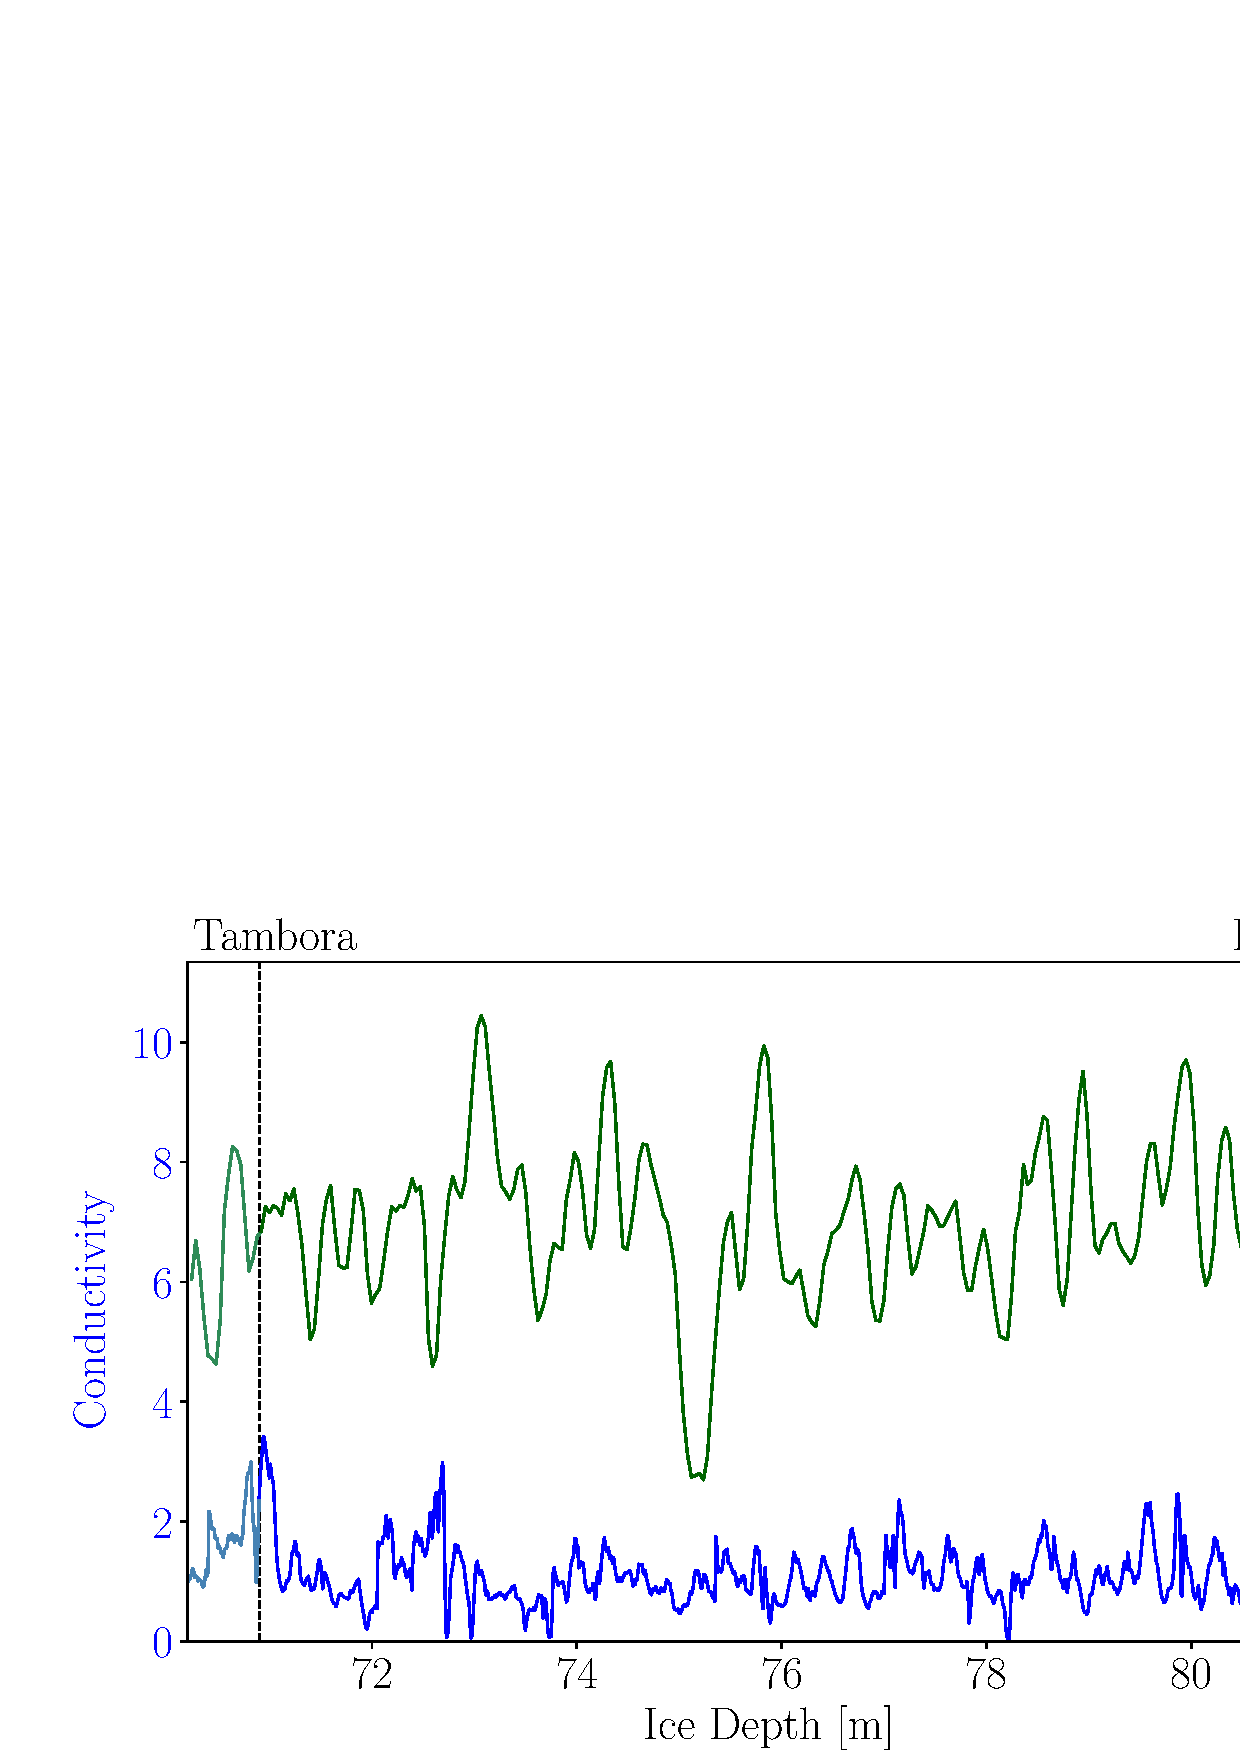
\includegraphics[width=0.7\textwidth]{SiteA_ECMd18O_combo.jpg}
	\caption[ECM and d18O data at LT, Site A.]{Two depth profiles from the core drilled at Site A showing accordingly the measured $\delta^{18}$O isotopic values and the conductivity measurements in the depth ranging from the estimated Tambora eruption to the Laki eruption.}	
	\label{fig:SiteA_ECMd18O_combo}
\end{figure}

\subsection[Preliminary Computations]{Preliminary Computations}
From the inputs a number of preliminary computations need to be carried out before the optimization of the diffusion length can be performed. For the depth series this consists of first interolating the data to make sure that the depth series is evenly sampled, then an analysis of signal and noise in the frequency spectrum needs to be carried out, and from this spectral analysis a Wiener filter can be constructed to find the optimal high frequency cut off, where as much noise as possible is filtered away while losing as little of the signal as possible. These computations are all based on the depth series data and use only signal analysis theory.\\
The input of core specifications on the other hand is used to give a more theoretical view of the situation. From these preliminary inputs, containing accumulation rate, borehole temperatures, altitudes and other conditions, it is possible to use ice core and ice flow theory to compute initial estimates of density and diffusion profiles at the given site. From these profiles along with the volcanic horizons indicating the series of interest, an initial estimate of the diffusion length at the depth of Laki to Tambora.\\
Firstly, the computations associated with inputted depth series are considered and later the ones associated with the core specifications are described. 
 
\subsubsection[Spline Interpolation]{Depth Series: Spline Interpolation}
When working with ice core data, it is not always a certainty that the data you get from the field are as continuous or as evenly sampled as one could have hoped. A lot of factors are at play when drilling, transporting, dividing and cutting an ice core for laboratory studies. Some parts of an ice core contain brittle zones where the ice is likely to break, leaving a section almost impossible to analyze. When transporting the drilled ice cores they are susceptible to both melting and contamination and evaporation of the outermost ice layer of the core. And finally of course there is a number of uncertainties that occur when cutting an ice core into discrete bits to be measured. The quality of data varies rather greatly from site to site, from drill team to drill team and of course from laboratory to laboratory. \\
When looking at the depth series only it might not be an issue to have various spacing between the discrete measurements, but when it comes to spectral analysis, it is of necessity to obtain a depth series signal with an even distribution. To accommodate this need interpolation of the signal can be of use. In the case of the ice core drilled at Site A, it can be seen from Figure \ref{fig:SiteA_d18OLT_Interp} that the raw measured signal has a minimum sampling size of $\Delta_{\text{min}}=0.038$ and a maximum sampling size of $\Delta_{\text{max}}=0.040$. To be able to analyze this signal in the spectral domain the signal can be numerically resampled with an even sampling rate. This is done by choosing the minimum sampling size available, $\Delta_{\text{min}}=0.038$, and redistributing the depth data points to be evenly spaced with this sampling size. The redistribution is carried out as follows.

Assuming the original depth array $\text{\textbf{d}}$ is distributed as $d_{i-1} < d_i < d_{i+1}$ with $i = 0, ..., n-1$ has a minimum sampling distance as $\Delta_{\text{min}}$ we define the new sampling distance for the new depth array $\hat{\text{\textbf{d}}}$ as $\Delta =\Delta_{\text{min}}$ - again assuming that $\hat{\text{\textbf{d}}}_{j-1} < \hat{\text{\textbf{d}}}_j < \hat{\text{\textbf{d}}}_{j+1}$ with $j = 0, ..., \hat{n}-1$. This makes it possible to define the first and last value of the new array as
\begin{equation}
	\hat{\text{d}}_0 = \Delta \lceil \frac{\text{d}_0}{\Delta}, \rceil 
	\label{Eq:InterpDepthMin}
\end{equation}
\begin{equation}
	\hat{\text{d}}_{\hat{n}-1} = \Delta \lfloor \frac{\text{d}_{n-1}}{\Delta} \rfloor.
	\label{Eq:InterpDepthMax}
\end{equation}
From this the number of values in the new array, $\hat{n}$, can be determined as
\begin{equation}
	\hat{n} = 1 +  \frac{\hat{\text{d}}_{\hat{n}-1} - \hat{\text{d}}_0}{\Delta},\;\;\;\;\; \hat{n} \in\mathbb{Z}.
\end{equation}
Thus our new depth array will be given as
\begin{equation}
	\hat{\text{\textbf{d}}} = \hat{\text{d}}_0 + j\cdot\Delta,\;\;\;\;\; j = 0, ..., \hat{n}-1.
\end{equation}
The original data are then used to define a cubic spline interpolation function to which the redistributed depth data points can be matched. For this part of the data analysis the \lstinline[columns=fixed]|SciPy.interpolate| Python (REFERENCE) package with \lstinline[columns=fixed]|SciPy.interpolate.CubicSpline| for the cubic spline interpolation. This gives a new distribution of data points as seen in Figure \ref{fig:SiteA_d18OLT_Interp}.


\begin{figure}[h]
	\centering
	\includegraphics[width=0.7\textwidth]{SiteA_d18OLT_Interp.jpg}
	\caption[Measured and interpolated $\delta^{18}$O data, Site A]{The unevenly measured data from Site A in the depth ranging from Tambora to Laki along with the now evenly sampled cubic spline interpolated data. Sampled with an interval of $\Delta = 0.038$.}
	\label{fig:SiteA_d18OLT_Interp}
\end{figure}

\subsubsection[Spectral Analysis]{Depth Series: Spectral Analysis}
Now with evenly spaced depth series data it is possible to transform the data to the frequency domain and perform spectral analysis on the signal. The basic theory concerning Fast Fourier Transform(FFT), Discrete Cosine Transform(DCT) and Power Spectral Densities(PSD) is discussed in Section \ref{Sec:????}. In this section the theory is merely put to use. Since the data under examination is completely real with no imaginary parts, pointing towards the sensibility of working only with cosines to enhance computational speed. Furthermore the DCT implies different boundary conditions than the FFT, meaning that some of the odd spectral behaviour, like aliasing can be avoided by using a different transform.\todo{Make a comment on Nyquist frequncy.}\\
For the depth series between Laki and Tambora at Site A, the PSD computed through the DCT as $\text{PSD} = |\text{DCT}|^2$ can be seen in Figure \ref{fig:SiteA_DCT_PSD_raw}. This spectrum shows a higher intensity in the low frequency area and a lower intensity at high frequencies indicating a low frequency signal and some high frequency noise.
\begin{figure}[h]
	\centering
	\begin{subfigure}{.45\textwidth}
		\centering
		\includegraphics[width=\textwidth]{SiteA_DCT_PSD_raw.jpg}
		\caption[PSD of LT data, Site A]{}
		\label{fig:SiteA_DCT_PSD_raw}
	\end{subfigure}
	~
	\begin{subfigure}{0.45\textwidth}
		\includegraphics[width=\textwidth]{SiteA_PSD_all}
		\caption[Spectral fit, Site A]{}%Signal(blue), noise(green) and fit(black).}
		\label{fig:SiteA_SpectralFitsAll}
	\end{subfigure}
	\caption[Spectral Analysis]{Spectral Analysis. \textbf{(a)} The power spectral density(PSD) of the interpolated data from Site A shown in Figure \ref{fig:SiteA_d18OLT_Interp}. The PSD was computed through a Discrete Cosine Transform(DCT). \textbf{(b)} Spectral estimate of the depth series from Tambora to Laki along with fit to entire spectral data set and the separated estimates of the noise and signal functions, as described in section \ref{sec:??}}
	\label{fig:SiteA_SpectralAnalysis}
\end{figure}

\begin{marginfigure}
	\centering
	\begin{subfigure}{\marginparwidth}
		\centering
		\includegraphics[width=\textwidth]{SiteA_PSD_sig.jpg}
		\caption{\footnotesize}
		\label{fig:SiteA_PSD_sig}
	\end{subfigure}\\[1ex]
	
	\begin{subfigure}{\marginparwidth}
		\centering
		\includegraphics[width=\textwidth]{SiteA_PSD_noise.jpg}
		\caption{\footnotesize}
		\label{fig:SiteA_PSD_noise}
	\end{subfigure}\\[1ex]
	
	\begin{subfigure}{\marginparwidth}
		\centering
		\includegraphics[width=\textwidth]{SiteA_PSD_fit.jpg}
		\caption{\footnotesize}
		\label{fig:SiteA_PSD_fit}
	\end{subfigure}
	\caption[Isolated spectral fits, Site A]{\footnotesize\textbf{(a)} Signal estimate given through fitting to all data (noise and signal). \textbf{(b)} Noise estimate given through fitting to all data (noise and signal). \textbf{(c)} Complete spectral fit to all data (blue), both noise and signal.}
	\label{fig:SpectralFitsIsolated}
\end{marginfigure}
Since the signal is that of a real physical phenomena, and even one that we do have some acquaintance with, it is relevant to use some of this knowledge to describe the apparent spectrum, which has also been done in section \ref{Sec:???}. Recalling the definitions of the noise and the signal as we assume them to be as:
\begin{equation}
	|\eta(\omega)|^2 = \frac{\sigma_{\eta}^2\Delta z}{|1+a_1\exp(-2\pi i \omega\Delta z)|^2}
	\label{Eq:MethodNoiseFit}
\end{equation}
\begin{equation}
	P_{\text{signal}} = P_0 \cdot e^{-k^2\sigma_{tot}^2}
	\label{Eq:MethodSignalFit}
\end{equation}
\todo{Write how the fitting routine is carried out. }The signal, noise and combined fit can be seen separately in Figure \ref{fig:SiteA_PSD_sig}, \ref{fig:SiteA_PSD_noise} and \ref{fig:SiteA_PSD_fit}, respectively, and plotted together in Figure \ref{fig:SiteA_SpectralAnalysis}.


\subsubsection[Wiener Filter]{Depth Series: Wiener Filter}
\begin{figure}[h]
	\centering
	\includegraphics[width=\textwidth]{SiteA_filtersEx.jpg}
	\caption[Frequency filters example, Site A]{Frequency filter examples ranging from diffusion length 0.04 m to 0.085 m.}
	\label{fig:SiteA_filtersEx}
\end{figure}

\subsubsection[Density Profile]{Core Specifications: Density Profile}
\begin{marginfigure}
	\centering
	\includegraphics[width=\marginparwidth]{SiteA_DensProfile_wHL.jpg}
	\caption[Density profile Site A]{\footnotesize{Depth density profile at Site A. Black is the measured densities during drilling, blue is the modelled density profile given a Herron Langway model, and orange is a Herron Langway model with a criterion to minimize the distance to the actual measurements.}}
	\label{Fig:SiteA_DensProfile_wHL}
\end{marginfigure}


\subsubsection[Diffusion Profile]{Core Specifications: Diffusion Profile}
\begin{marginfigure}
	\centering
	\includegraphics[width=\marginparwidth]{SiteA_DiffProfile.jpg}
	\caption[Diffusion profile, Site A.]{\footnotesize{Estimated diffusion profile at Site A given a Herron Langway model.}}
	\label{fig:SiteADiffProfile}
\end{marginfigure}

\subsubsection[$\sigma_0$ estimate]{Core Specifications: $\sigma_0$ estimate}

\subsection[Back Diffusion]{Back Diffusion/Deconvolution}

\subsection[Peak Counting]{Peak Counting}

\subsection[Decision algorithm]{Decision Algorithm}

\subsection[Output]{Output}


\begin{figure}
	\centering
	\includegraphics[width=0.7\textwidth]{SiteA_BackDiffused_Y32.jpg}
	\caption[Best estimate of deconvoluted depth series, Site A]{Best estimate of deconvoluted depth series given an annual count of 32 years - marked as orange dots. The best estimate is taken as the largest diffusion length that still yields 32 years in the depth span from Tambora to Laki.}
	\label{fig:SiteA_BackDiffused_Y32}
\end{figure}

\begin{figure}
	\centering
	\includegraphics[width=\textwidth]{SiteA_BackDiffused_AllSigmaEst.jpg}
	\caption[All diffusion length estimate deconvolutions, Site A]{Estimated back diffused data series with different diffusion length estimates: diffusion length estimate from spectral fit ($\sigma_{fit}$), maximum ($\sigma_{Max}^{Theo}$) and minimum ($\sigma_{Min}^{Theo}$) theoretically estimated diffusion lengths and final estimated diffusion length.}
	\label{fig:SiteA_BackDiffused_AllSigmaEst}
\end{figure}















\end{document}
